\section{Ice Model Formulation}
\label{Iphys}

The sea-ice component of ROMS is a combination of the
elastic-viscous-plastic (EVP) rheology (
\cite{Hunke97}, \cite{Hunke_2001}) and simple one-layer
ice and snow thermodynamics with a molecular sublayer under the ice
(\cite{Mellor89}). It is tightly coupled, having
the same grid (Arakawa-C) and timestep as the ocean and sharing the same
parallel coding structure for use with MPI or OpenMP (\cite{Budgell05}).

\subsection{Dynamics}
The momentum equations describe the change in ice/snow velocity due
to the combined effects of the Coriolis force, surface ocean tilt,
air and water stress, and internal ice stress:
(\ref{ist1}) and (\ref{ist2}):
\begin{align}
  M \frac{\partial u }{ \partial t}
 % + M \vec{v} \cdot \nabla u
 & = Mfv - Mg \frac{\partial \zeta_w }{ \partial x} +
 \tau_a^x + \tau_w^x + {\cal F}_x
\label{ist1} \\
  M \frac{\partial v }{ \partial t}
 % + M \vec{v} \cdot \nabla v
 & = - Mfu - Mg \frac{\partial \zeta_w }{ \partial y} +
 \tau_a^y + \tau_w^y + {\cal F}_y.
\label{ist2}
\end{align}
In this model, we neglect the nonlinear advection terms as well as
the curvilinear terms in the internal ice stress.
Nonlinear formulae are used for both the ocean-ice and air-ice surface
stress:
\begin{align}
  \vec{\tau}_a & = \rho_a C_a | \vec{V}_{10} | \vec{V}_{10} \\
  C_a & = \frac{1 }{ 2} C_d \left[ 1 - \cos( 2 \pi \min(h_i+.1, .5)
  \right] \\
  \vec{\tau}_w & = \rho_w C_w | \vec{v}_w - \vec{v} |
  ( \vec{v}_w - \vec{v}) .
\end{align}
The force due to
the internal ice stress is given by the divergence of the stress
tensor $\sigma$. The rheology is given by the stress-strain relation
of the medium. We would like to emulate the viscous-plastic rheology
of \cite{Hibler79}:
\begin{equation}
  \sigma_{ij} = 2 \eta \dot \epsilon_{ij} + (\zeta - \eta) \dot
  \epsilon_{kk} \delta_{ij} - \frac{P }{ 2} \delta_{ij}
\end{equation}
\begin{equation}
  \dot \epsilon_{ij} \equiv \frac{1 }{ 2} \left( \frac{\partial u_i
  }{
  \partial x_j} + \frac{\partial u_j }{ \partial x_i} \right)
\end{equation}
\begin{equation}
  P = P^* A h_i e^{-C(1-A)}
\end{equation}
where the nonlinear viscosities are given by
\begin{equation}
\zeta = \frac{ P }{ 2 \left[ (\epsilon^2_{11} +
   \epsilon^2_{22} ) ( 1 + 1/e^2 ) + 4 e^{-2} \epsilon^2_{12}
      + 2 \epsilon_{11} \epsilon_{22} ( 1 - 1/e^2 ) \right] ^{1/2} }
\end{equation}
\begin{equation}
      \eta = \frac{ \zeta }{ e^2 }.
\end{equation}
We would also like to have an explicit model that can be solved
efficiently on parallel computers. The EVP rheology has a tunable
coefficient $E$ (the Young's modulus) which can be chosen to make
the elastic term small compared to the other terms. We rearrange the VP
rheology:
\begin{equation}
  \frac{1 }{ 2 \eta} \sigma_{ij} + \frac{\eta - \zeta }{ 4 \eta \zeta}
  \sigma_{kk} \delta_{ij} + \frac{P }{ 4 \zeta} \delta_{ij} = \dot
  \epsilon_{ij}
\end{equation}
then add the elastic term:
\begin{equation}
  \frac{1 }{ E} \frac{\partial \sigma_{ij} }{ \partial t} +
  \frac{1 }{ 2
  \eta} \sigma_{ij} + \frac{\eta - \zeta }{ 4 \eta \zeta} \sigma_{kk}
  \delta_{ij} + \frac{P }{ 4 \zeta} \delta_{ij} = \dot \epsilon_{ij}
\end{equation}

Much like the ocean model, the ice model has a split timestep. The
internal ice stress term is updated on a shorter timestep so as to
allow the elastic wave velocity to be resolved.

Once the new ice velocities are computed, the ice tracers can be
advected using the MPDATA scheme \cite{Smolark90}. The tracers in
this case are the ice thickness, ice concentration, snow thickness,
internal ice temperature, and surface melt ponds. The continuity
equations describing the evolution of these parameters (equations
(\ref{ist3a})--(\ref{ist3b})) also include thermodynamic terms ($S_h$,
$S_s$ and $S_A$), which will be described in \S\ref{Growth}:
\begin{align}
  \frac{\partial A h_i }{ \partial t} & =
  - \frac{\partial (u A h_i) }{ \partial x} -
  \frac{\partial (v A h_i) }{ \partial y}
  + S_h + {\cal D}_h
\label{ist3a} \\
  \frac{\partial A h_s }{ \partial t} & =
  - \frac{\partial (u A h_s) }{ \partial x} -
  \frac{\partial (v A h_s) }{ \partial y}
  + S_s + {\cal D}_s
\label{ist3c} \\
  \frac{\partial A }{ \partial t} & =
  - \frac{\partial (uA) }{ \partial x} - \frac{\partial (vA) }{ \partial y}
  + S_A + {\cal D}_A \qquad \qquad 0 \leq A \leq 1 .
\label{ist3b}
\end{align}
The first two equations represent the conservation of ice and snow.
Equation \ref{ist3b} is discussed in some detail in MK89, but
represents the advection of ice blocks in which no ridging occurs as
long as there is any open water.
%An optional ridging term can be added
%(\cite{Gray96}):
%\begin{equation}
%  \frac{\partial A }{ \partial t} =
%  - \frac{\partial (uA) }{ \partial x} - \frac{\partial (vA) }{ \partial y}
%  - A \alpha(A) \, \nabla \cdot \vec{v} \, H(-\nabla \cdot \vec{v})
%  + S_A + {\cal D}_A \qquad \qquad 0 \leq A \leq 1 .
%\end{equation}
%where $\alpha(A)$ is an arbitrary function such that $\alpha(0) = 0$,
%$\alpha(1) = 1$, and $0 \leq \alpha(A) \leq 1$. The ridging term leads
%to an increase in $h_i$ under convergent flow as would be produced by
%ridging. The function $\alpha(A)$ should be chosen so that it is near
%zero until the ice concentration is large enough that ridging is
%expected to occur, then should increase smoothly to one.
%
The symbols used in these equations along with the values for the
constants are listed in Table \ref{icemomvars}.

\begin{table}[pt]
\hspace{9.5 mm}
\vbox{
\begin{tabular}{|c|c|l|} \hline
  Variable & Value & Description \\ \hline
  $A(x,y,t)$ && ice concentration \\
%  $\alpha(A)$ && ridging function \\
  $C_a$ && nonlinear air drag coefficient \\
  $C_d$ & $2.2 \times 10^{-3}$ & air drag coefficient \\
  $C_w$ & $10 \times 10^{-3}$ & water drag coefficient \\
  (${\cal D}_h, {\cal D}_s, {\cal D}_A$) && diffusion terms \\
  $\delta_{ij}$ && Kronecker delta function \\
  $E$ && Young's modulus \\
  $e$ & 2 & eccentricity of the elliptical yield curve \\
  $\epsilon_{ij}(x,y,t)$ && strain rate tensor \\
  $\eta(x,y,t)$ && nonlinear shear viscosity \\
  $f(x,y)$ && Coriolis parameter \\
  (${\cal F}_x, {\cal F}_y$) && internal ice stress \\
  $g$  & $9.8\, m\, s^{-2}$ & acceleration of gravity \\
  $H$ &&  Heaviside function \\
  $h_i(x,y,t)$ && ice thickness of ice-covered fraction \\
  $h_o$ & 1 m & ice cutoff thickness \\
  $h_s(x,y,t)$ && snow thickness on ice-covered fraction \\
  $M(x,y,t)$ && ice mass (density times thickness) \\
  $P(x,y,t)$ && ice pressure or strength \\
  ($P^*, C$) & ($2.75 \times 10^4, 20$) & ice strength parameters \\
  ($S_h, S_s, S_A$) && thermodynamic terms \\
  $\sigma_{ij}(x,y,t)$ && stress tensor \\
  $\vec{\tau}_a$ && air stress \\
  $\vec{\tau}_w$ && water stress \\
  ($u,v$) && the ($x,y$) components of ice velocity $\vec{v}$ \\
  ($\vec{V}_{10}, \vec{v}_w$) &&
	      10 meter air and surface water velocities \\
  ($\rho_a, \rho_w$)  & ($1.3\, kg\, m^{-3}, 1025\, kg\, m^{-3}$) & air
  and water densities \\
  $\zeta(x,y,t)$ && nonlinear bulk viscosity \\
  $\zeta_w(x,y,t)$ && height of the ocean surface \\
  \hline
\end{tabular}
}
\caption{Variables used in the ice momentum equations}
\label{icemomvars}
\end{table}

Note that Hibler's $h_I$ variable is equivalent to our $A h_i$
combination - his $h_I$ is the average thickness over the whole
gridbox while our $h_i$ is the average thickness over the ice-covered
fraction of the gridbox. 

\subsection{Thermodynamics}
\label{Growth}

The thermodynamics is based on calculating how much ice grows and
melts on each of the surface, bottom, and sides of the ice floes,
as well as frazil ice formation (\cite{Mellor89}).
Once the ice tracers are advected, the ice concentration and
thickness are timestepped according to the terms on the right:

Equations (\ref{ist3a}) and (\ref{ist3b}) become:
\begin{align}
  \frac{D A h_i }{D t}
  & = \frac{\rho_o }{ \rho_i} \left[ A (W_{io} - W_{ai}) + (1-A) W_{ao}
  + W_{fr} \right]
\label{ist4a} \\
  \frac{D A }{ D t}
  & = \frac{\rho_o A }{ \rho_i h_i} \left[ \Phi (1-A) W_{ao} + (1-A)
  W_{fr} \right] \qquad \qquad 0 \leq A \leq 1 .
\label{ist4b}
\end{align}
The term $Ah_i$ is the ``effective thickness'', a measure of the ice
volume. Its evolution equation is simply quantifying the change in
the amount of ice. The ice concentration equation is more interesting in
that it provides the partitioning between ice melt/growth on the sides
vs. on the top and bottom. The parameter $\Phi$ controls this and has
differing values for ice melt and retreat. In principle, most of the ice
growth is assumed to happen at the base of the ice while rather more of
the melt happens on the sides of the ice due to warming of the water in
the leads.

The heat fluxes through the ice are based on a simple one layer
\cite{Semtner76a} type model with snow on top. The temperature is
assumed to be linear within the snow and within the ice. The ice contains
brine pockets for a total ice salinity of 3.2 or the surface salinity,
whichever is less. The surface ocean temperature and salinity is half a
$dz$ below the surface. The water right below the surface is assumed to
be at the freezing temperature; a logarithmic boundary layer is computed
having the temperature and salinity matched at freezing.

Here, the $W$ variables are the freeze or
melt rates as shown in Fig.\ \ref{fm+k} and Table \ref{thermvar}.  The
frazil ice growth $W_{fr}$ will be discussed further in
\S\ref{frazil}---note that it contributes to changes in $A$ as well as
to changes in $h_i$.  The other term that contributes to $A$ is
$W_{ao}$.  This term includes a factor $\Phi$ which Mellor and Kantha
set to different values depending on whether ice is melting or
freezing:
\begin{align}
    \Phi & = 4.0 \qquad\qquad W_{ao} \geq 0 \\
    \Phi & = 0.5 \qquad\qquad W_{ao} < 0 \\
\end{align}

\begin{figure}[ht]
\setlength{\unitlength}{0.00083300in}%
%
%\begin{picture}(6527,2507)(270,-5042)
\begin{picture}(6591,3076)(835,-5072)
%\thicklines
\put(1501,-2911){\line( 1, 0){3975}}
\put(1501,-4111){\line( 1, 0){3975}}
\put(1501,-2911){\line( 0,-1){1200}}
\put(6976,-4111){\line( 1, 0){1050}}
\put(6976,-2941){\line( 1, 0){1050}}
\put(6976,-2711){\line( 0,-1){1400}}
\put(6976,-2711){\line( 1, 0){1050}}
\put(5476,-2911){\line( 0,-1){1200}}
\put(2401,-4811){\vector( 0, 1){700}}
\put(3376,-4861){\vector( 0, 1){750}}
\put(6226,-3586){\vector( 0, 1){675}}
\put(4426,-4036){\vector( 0,-1){525}}
\put(2596,-3376){\vector( 1, 1){450}}
\put(7526,-2211){\vector( 0,-1){500}}
\put(7490,-3383){\vector( 1,2){200}}
\put(6121,-3786){\makebox(0,0)[lb]{$W_{ao}$}}
\put(4336,-4756){\makebox(0,0)[lb]{$W_{ro}$}}
\put(2416,-3586){\makebox(0,0)[lb]{$W_{ai}$}}
\put(3241,-5056){\makebox(0,0)[lb]{$W_{io}$}}
\put(2296,-5056){\makebox(0,0)[lb]{$W_{fr}$}}
\put(7400,-2180){\makebox(0,0)[lb]{$W_{s}$}}
\put(7276,-3611){\makebox(0,0)[lb]{$W_{sm}$}}
\end{picture}
%\begin{picture}(0,0)(5346,0)
\begin{picture}(0,0)(5961,-30)
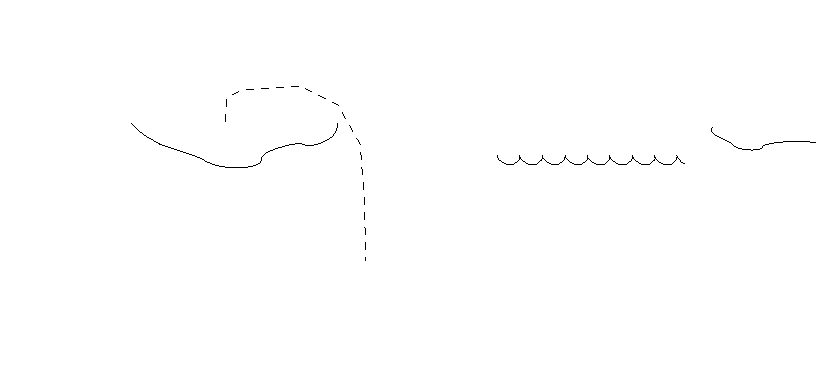
\includegraphics{pics/therm_mk}%
\end{picture}%
\caption{Diagram of the different locations where ice melting and
freezing can occur.}
\label{fm+k}
\end{figure}

Similar to Eq. \ref{ist4a} is the snow equation:
\begin{equation}
  {D A h_s \over D t} = \left[ A (W_{s} - W_{sm}) \right]
\end{equation}
where $W_s$ and $W_{sm}$ are the snowfall and snow melt rates,
respectively, in units of equivalent water. Also in the model is
the depth of the melt ponds in spring, $h_{mp}$ which can be up to
0.1 m, after which melting ice contributes to $W_{ro}$. The melt
ponds are not part of the thermal conductivity computations. They
could contribute to the albedo computation, but that has been
largely commented out.

\begin{table}
\hspace{9 mm}
\vbox{
\begin{tabular}{|c|c|l|} \hline
  Variable & Value & Description \\ \hline
  $\alpha_w$ & 0.10 & shortwave albedo of water \\
  $\alpha_i$ & 0.60 & shortwave albedo of wet ice \\
  $\alpha_i$ & 0.65 & shortwave albedo of dry ice \\
  $\alpha_s$ & 0.72 & shortwave albedo of wet snow \\
  $\alpha_s$ & 0.85 & shortwave albedo of dry snow \\
  $C_k$ && snow correction factor \\
  $C_{pi}$ & 2093 J kg$^{-1}$ K$^{-1}$ & specific heat of ice \\
  $C_{po}$ & 3990 J kg$^{-1}$ K$^{-1}$ & specific heat of water \\
  $\epsilon_w$ & 0.97 & longwave emissivity of water \\
  $\epsilon_i$ & 0.97 & longwave emissivity of ice \\
  $\epsilon_s$ & 0.99 & longwave emissivity of snow \\
  $E(T,r)$ && enthalpy of the ice/brine system \\
  $F_T\!\uparrow$ && heat flux from the ocean into the ice \\
  $H\!\downarrow$ && sensible heat \\
  $i_w$ && fraction of the solar heating transmitted \\
  && through a lead into the water below \\
  $k_i$ & 2.04 W m$^{-1}$ K${^-1}$ & thermal conductivity of ice \\
  $k_s$ & 0.31 W m$^{-1}$ K${^-1}$ & thermal conductivity of snow \\
  $L_i$ & 302 MJ m$^{-3}$ & latent heat of fusion of ice \\
  $L_s$ & 110 MJ m$^{-3}$ & latent heat of fusion of snow \\
  $LE\!\downarrow$ && latent heat \\
  $LW\!\!\downarrow$ && incoming longwave radiation \\
  $m$ & $-0.054^\circ$C/PSU & coefficient in linear $T_f(S) = mS$ equation \\
  $\Phi$ && contribution to $A$ equation from freezing water \\
  $Q_{ai}$ && heat flux out of the snow/ice surface \\
  $Q_{ao}$ && heat flux out of the ocean surface \\
  $Q_{i2}$ && heat flux up out of the ice \\
  $Q_{io}$ && heat flux up into the ice \\
  $Q_{s}$  && heat flux up through the snow \\
  $r$   & $0 \le r \le 0.2 $ & brine fraction in ice \\
  $\rho_i$ & 910 $m^3/kg$ & density of ice \\
  $S_i$ & 3.2 PSU & salinity of the ice \\
  $SW\!\!\downarrow$ && incoming shortwave radiation \\
  $\sigma$ & $5.67 \times 10^{-8}$ W m$^{-2}$ K$^{-4}$ &
  Stefan-Boltzmann constant \\
  $T_0$ && temperature of the bottom of the ice \\
  $T_1$ && temperature of the interior of the ice \\
  $T_2$ && temperature at the upper surface of the ice \\
  $T_3$ && temperature at the upper surface of the snow \\
  $T_f$ && freezing temperature \\
  $T_{{\rm melt}\_i}$ & $mS_i$ & melting temperature of ice \\
  $T_{{\rm melt}\_s}$ & 0$^\circ$ C & melting temperature of snow \\
  $W_{ai}$ && melt rate on the upper ice/snow surface \\
  $W_{ao}$ && freeze rate at the air/water interface \\
  $W_{fr}$ && rate of frazil ice growth \\
  $W_{io}$ && freeze rate at the ice/water interface \\
  $W_{ro}$ && rate of run-off of surface melt water \\
  $W_{s}$  && snowfall rate \\
  $W_{sm}$ && snow melt rate \\
  \hline
\end{tabular}
}
\caption{Variables used in the ice thermodynamics}
\label{thermvar}
\end{table}

\begin{figure}
\centerline{
\begin{picture}(0,0)%
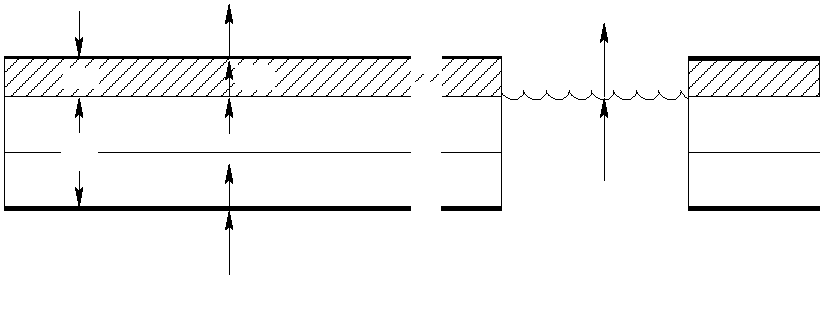
\includegraphics{pics/therm_mk2}%
\end{picture}%
\setlength{\unitlength}{3947sp}%
%
\begin{picture}(6591,2608)(1468,-5057)
\put(6376,-3511){\makebox(0,0)[lb]{{$F_T$}}}
\put(3376,-4561){\makebox(0,0)[lb]{{$F_T$}}}
\put(3376,-4036){\makebox(0,0)[lb]{{$Q_{io}$}}}
\put(3376,-3436){\makebox(0,0)[lb]{{$Q_{i2}$}}}
\put(6376,-3061){\makebox(0,0)[lb]{{$Q_{ao}$}}}
\put(3376,-3136){\makebox(0,0)[lb]{{$Q_s$}}}
\put(3376,-2761){\makebox(0,0)[lb]{{$Q_{ai}$}}}
\put(2026,-3736){\makebox(0,0)[lb]{{$h_i$}}}
\put(2026,-3136){\makebox(0,0)[lb]{{$h_s$}}}
\put(4801,-4186){\makebox(0,0)[lb]{{$T_0$}}}
\put(4801,-2986){\makebox(0,0)[lb]{{$T_3$}}}
\put(4801,-3286){\makebox(0,0)[lb]{{$T_2$}}}
\put(4801,-3736){\makebox(0,0)[lb]{{$T_1$}}}
\end{picture}
}
\caption{Diagram of internal ice temperatures and fluxes. The hashed
layer is the snow.}
\label{fflux}
\end{figure}

Figure \ref{fflux} shows the locations of the ice and snow temperatures
and the heat fluxes. The temperature profile is assumed to be linear
between adjacent temperature points. The interior of the ice contains
``brine pockets'', leading to a prognostic equation for the temperature
$T_1$.

The surface flux to the air is:
\begin{equation}
   Q_{ai} =  - H\!\downarrow - LE\!\downarrow -
       \epsilon_s LW\!\!\downarrow  -
      (1 - \alpha_s) SW\!\!\downarrow + \epsilon_s \sigma (T_3+273)^4
\end{equation}
The incoming shortwave and longwave radiations are assumed to
come from an atmospheric model. The formulae for sensible heat,
latent heat, and outgoing longwave radiation are the same as in
\cite{Parkinson} and are shown in Appendix
\ref{shortwave}. The sensible heat is a function of $T_3$, as is the
heat flux through the snow $Q_s$. Setting $Q_{ai} = Q_s$, we can solve
for $T_3$ by setting $T_3^{n+1} = T_3^n + \Delta T_3$ and linearizing in
$\Delta T_3$. As in Parkinson and Washington, if $T_3$
is found to be above the melting temperature, it is set to $T_{\rm melt}$
and the extra energy goes into melting the snow or ice:
\begin{align}
   W_{ai} & = \frac{Q_{ai} - Q_{i2} }{ \rho_o L_3} \\
   L_3 & \equiv \left[ E(T_3,1) - E(T_1, R_1) \right]
\end{align}
Note that $L_3 = (1-r)L_i$ plus a small sensible heat correction.
We can store water on the surface in melt pools to a fixed
depth---everything extra melted at the surface is assumed to flow into
the ocean as $W_{ro}$. The melt ponds however do not contribute to
the heat flux computation.

Inside the ice there are brine pockets in which there is salt water
at the {\it in situ} freezing temperature. It is assumed that the ice
has a uniform overall salinity of $S_i$ and that the freezing
temperature is a linear function of salinity. The brine fraction $r$ is
given by
$$
  r = \frac{S_i m }{ T_1}
$$
The enthalpy of the combined ice/brine system is given by
\begin{equation}
  E(T,r) = r(L_i + C_{po}T) + (1-r) C_{pi} T
\end{equation}
Substituting in for $r$ and differentiating gives:
\begin{equation}
  \frac{\partial E }{ \partial T} = - \frac{S_i m L_i }{ T_1^2} + C_{pi}
\end{equation}

Inside the snow, we have
\begin{equation}
   Q_s = \frac{k_s }{ h_s} (T_2 - T_3)
\end{equation}
The heat conduction in the upper part of the ice layer is
\begin{equation}
   Q_{I2} = \frac{ 2 k_i }{ h_i} (T_1 - T_2)
   \label{qi2}
\end{equation}
These can be set equal to each other to solve for $T_2$
\begin{equation}
   T_2 = \frac{T_3 + C_k T_1 }{ 1 + C_k}
\end{equation}
where
$$
  C_k \equiv \frac{2 k_i h_s }{ h_i k_s}.
$$
Substituting into (\ref{qi2}), we get:
\begin{equation}
  Q_s = Q_{I2} = \frac{2k_i }{ h_i} \frac{(T_1 - T_3) }{ (1 + C_k)}
\label{qsnow}
\end{equation}
Note that in the absence of snow, $C_k$ becomes zero and we recover the
formula for the no-snow case in which $T_3 = T_2$.

At the bottom of the ice, we have
\begin{equation}
  Q_{I0} = \frac{2 k_i }{ h_i} (T_0 - T_1)
\end{equation}
The difference between $Q_{I0}$ and $Q_{I2}$ goes into the enthalpy of
the ice:
\begin{equation}
   \rho_i h_i \left[ \frac{\partial E }{ \partial t} + \vec{v} \cdot 
   \nabla E \right] = Q_{I0} - Q_{I2}
\end{equation}
We can use the chain rule to obtain an equation for timestepping $T_1$:
\begin{equation}
   \rho_i h_i \frac{\partial E }{ \partial T}
   \left[ \frac{\partial T_1 }{ \partial t} + \vec{v} \cdot 
   \nabla T_1 \right] = Q_{I0} - Q_{I2}
\end{equation}
where
\begin{align*}
  Q_{I0} - Q_{I2} & = \frac{2 k_i }{ h_i} \left[ (T_0 - T_1) - 
  \frac{(T_1 - T_3) }{ 1 + C_k} \right] \\
	          & = \frac{2 k_i }{ h_i} \left[ (T_0 +
  \frac{T_3 - (2 + C_k) T_1 }{ 1 + C_k} \right]
\end{align*}

\subsubsection{Ocean surface boundary conditions}
The ocean receives surface stresses from both the atmosphere and the
ice, according to the ice concentration:
\begin{align}
   K_m \frac{\partial u_w }{ \partial z} & = \frac{A }{ \rho_o} \tau_{io}^x
    + \frac{1-A }{ \rho_o} \tau_{ao}^x \\
   K_m \frac{\partial v_w }{ \partial z} & = \frac{A }{ \rho_o} \tau_{io}^y
    + \frac{1-A }{ \rho_o} \tau_{ao}^y
\end{align}
where the relevant variables are in table \ref{tobc}.

\begin{table}
\hspace{35 mm}
\vbox{
\begin{tabular}{|c|c|l|} \hline
Variable & Value & Definition \\ \hline
   $b$ & 3.14 & factor \\
   \.E && evaporation \\
   $k$ & 0.4 & von Karman's constant \\
   $K_m$ && vertical viscosity of seawater \\
   $\nu$ & $1.8 \times 10^{-6} m^2 s^{-1}$ &
      kinematic viscosity of seawater \\
   \.P && precipitation \\
   $Pr$ & 13.0 & molecular Prandtl number \\
   $P_{rt}$ & 0.85 & turbulent Prandtl number \\
   $S$ && internal ocean salinity \\
   $S_0$ && surface salinity \\
   $Sc$ & 2432.0 & molecular Schmidt number \\
   $\tau_{io}$ && stress on the ocean from the ice \\
   $\tau_{ao}$ && stress on the ocean from the wind \\
   $T$ && internal ocean temperature \\
   $T_0$ && surface temperature \\
   $u_\tau$ && friction velocity $|\tau_{io}|^{1/2} \rho_o^{-1/2}$ \\
   $z_0$ && roughness parameter \\
  \hline
\end{tabular}
}
\caption{Ocean surface variables}
\label{tobc}
\end{table}

The surface ocean is assumed to be at the freezing temperature for the
surface salinity ($T_0 = mS_0$) in the presense of ice. We also have $T$ and $S$ at the
uppermost computed ocean point ${1 \over 2} dz$ below the surface.
In order to solve for $T_0$ and $S_0$, we assume a (\cite{Yaglom_1974})
logarithmic boundary layer. The upper ocean heat flux is:
\begin{equation}
   \frac{F_T }{ \rho_o C_{po}} = -C_{T_z} (T_0 - T) \qquad z \rightarrow 0
\end{equation}
where
\begin{gather}
  C_{T_z} = \frac{u_\tau }{ P_{rt} k^{-1}\ln (-z/z_0) + B_T} \\
  B_T = b \left(\frac{z_0 u_\tau }{ \nu} \right) ^{1/2} Pr^{2/3}
\end{gather}
Likewise, we have the following equation for the surface salt flux:
\begin{equation}
   F_S = -C_{S_z} (S_0 - S) \qquad z \rightarrow 0
\end{equation}
where
\begin{gather}
  C_{S_z} = \frac{u_\tau }{ P_{rt} k^{-1}\ln (-z/z_0) + B_S} \\
  B_S = b \left(\frac{z_0 u_\tau }{ \nu} \right) ^{1/2} Sc^{2/3}
\end{gather}

The ocean model receives the following heat and salt fluxes:
\begin{align}
   F_T & = A Q_{io} + (1 - A) Q_{ao} - W_o L_o \\
   F_S & = (W_o - A W_{ro}) (S_i-S_0) + (1-A)S_o (\mbox{\.P}-\mbox{\.E}) \\
   W_o & \equiv A W_{io} + (1-A) W_{ao}
\end{align}

(\cite{Mellor89}) describe solving simultaneously for
the five unknowns $W_o$, $T_0$, $S_0$, $F_T$ and $F_S$. Instead, we use
the old value of $T_0$ to find $W_{io}$ and therefore $W_o$. Using the
new value of $W_{io}$, solve for a new value of $S_0$ and then find the
new $T_0$ as the freezing temperature for that salinity:
\begin{align}
   W_{io} &= {1 \over L_o} \left[ {Q_{io} \over \rho_o} + C_{po}
   C_{T_z} (T_o - T) \right] \\
   S_0 &= { C_{S_z} S + (W_{ai}H(-W_{ai}) - W_{io})) S_i \over
   C_{S_z} + W_{ai}H(-W_{ai}) + W_{ro} - W_{io} }
\end{align}
Note that the term $W_{ai}H(-W_{ai})$ is the contribution of melting
only, not refreezing of melt ponds.

%Once we have a the value for $F_T$, we can use it to find the ice
%growth rates:
%\begin{align}
%   W_{io} &= \frac{1 }{ \rho_o L_o} (Q_{io} - F_T) \\
%   W_{ao} &= \frac{1 }{ \rho_o L_o} (Q_{ao} - F_T) \\
%\end{align}
%where
%\begin{equation}
%   L_o \equiv \left[ E(T_0,1) - E(T_1,r_1) \right]
%\end{equation}

\subsubsection{Frazil ice formation}
\label{frazil}

Following \cite{Steele89}, we check to see if any
of the ocean temperatures are below freezing at the end of each
timestep.  If so, frazil ice is formed, changing the local
temperature and salinity.  The ice that forms is assumed to
instantly float up to the surface and add to the ice layer there.
We balance the mass, heat, and salt before and after the ice
is formed:
\begin{align}
   m_{w_1} & = m_{w_2} + m_i \\
   m_{w_1} ( C_{pw} T_1 + L) & =
   m_{w_2} (C_{pw} T_2 + L) + m_i C_{pi} T_2 \\
   m_{w_1} S_1 & = m_{w_2} S_2 .
\end{align}
The variables are defined in Table \ref{frazvar}.
\begin{table}[t]
\hspace{35 mm}
\vbox{
\begin{tabular}{|c|c|l|} \hline
Variable & Value & Definition \\ \hline
   $C_{pi}$ & 1994 J kg$^{-1}$ K$^{-1}$ & specific heat of ice \\
   $C_{pw}$ & 3987 J kg$^{-1}$ K$^{-1}$ & specific heat of water \\
   $\gamma$ & $m_i/m_{w_2}$ & fraction of water that froze \\
   $L$ & 3.16e5 J kg$^{-1}$ & latent heat of fusion \\
   $m_i$ && mass of ice formed \\
   $m_{w_1}$ && mass of water before freezing \\
   $m_{w_2}$ && mass of water after freezing \\
   $m$ & $-0.0543$ & constant in freezing equation \\
   $n$ & $7.59 \times 10^{-4}$ & constant in freezing equation \\
   $S_1$ && salinity before freezing \\
   $S_2$ && salinity after freezing \\
   $T_1$ && temperature before freezing \\
   $T_2$ && temperature after freezing \\
  \hline
\end{tabular}
}
\caption{Frazil ice variables}
\label{frazvar}
\end{table}
Defining $\gamma = m_i / m_{w_2}$ and dropping terms of order $\gamma^2$
leads to:
\begin{align}
   T_2 & = T_1 + \gamma \left[ \frac{L }{ C_{pw}} + T_1 \left( 1
   - \frac{C_{pi} }{ C_{pw}} \right) \right] \label{t2eq} \\
   S_2 & = S_1 (1 + \gamma) \label{s2eq} .
\end{align}
We also want the final temperature and salinity to be on the freezing
line, which we approximate as:
\begin{equation}
   T_f = m S + n z .
\end{equation}
We can then solve for $\gamma$:
\begin{equation}
   \gamma = \frac{-T_1 + mS_1 + nz }{ {L }{ C_{pw}}+ T_1 \left( 1
   - \frac{C_{pi} }{ C_{pw}} \right) - mS_1} .
\end{equation}
The ocean is checked at each depth $k$ and at each timestep for
supercooling.  If the water is below freezing, the temperature and
salinity are adjusted as in equations (\ref{t2eq}) and (\ref{s2eq})
and the ice above is thickened by the amount:
\begin{equation}
   \Delta h = \gamma_k \Delta z_k \frac{\rho_w}{\rho_i} .
\end{equation}

\subsubsection{Differences from Mellor and Kantha}
We have tried to modify the \code{hakkis} model to more closely follow
MK89. However, there are also ways in which we have deviated from it.
\begin{itemize}
  \item Add advection of snow.
  \item Add lateral melting of snow when ice is melting laterally.
%  \item We iterate on the solution of $T_3$.
%  \item We took a shortcut in the solution of $S_0, T_0$ for the
%    surface heat and salt fluxes. We also apply them differently to the
%    ocean model.
  \item Add various limiters:
    \begin{itemize}
      \item Ice concentration:$A_{\min} \leq A \leq 1.0$, $A_{\min} = 0.0$.
      \item Ice thickness: $h_i \geq 0.0$.
      \item Snow thickness: $h_s \geq 0.0$.
      \item Brine fraction: $r \leq r_{\max}$, $r_{\max} = 0.2$
     \item Surface water: $0.0 \leq W_s \leq W_{s\max}$, $W_{s\max} = 0.1$
    \end{itemize}
\end{itemize}
